% Appendix: after \bibliography. Unlimited pages; reviewers are not required to read it.
\appendix

\section{Additional Implementation Details}
\label{app:impl}

We list the score mapping $M$ and the critic prompts for $F_{\mathrm{part}}$, $F_{\mathrm{ref}}$, $F_{\mathrm{act}}$, $F_{\mathrm{grp}}$, and $F_{\mathrm{rev}}$.

\subsection{Score mapping}
\label{app:score-map}

Table~\ref{tab:score-map} maps the two labels to a scalar in $\{0,0.2,0.4,0.6,0.8,1.0\}$.
The same table is used at both levels: $e_t$/$e_k$ as execution or subgoal status, and $p_t$/$p_k$ as subgoal or task contribution.

\begin{table}[h]
\caption{Lookup table $M$ mapping the two labels to a scalar. The same table is used at both the action level and the group level.}
\label{tab:score-map}
\centering
\small
\begin{tabular}{lcccc}
\toprule
Contribution & Completed & Partial & Failed & Uncertain \\
\midrule
Milestone & $1.0$ & $0.4$ & $0.0$ & $0.4$ \\
Useful-efficient & $0.8$ & $0.4$ & $0.0$ & $0.4$ \\
Useful-inefficient & $0.6$ & $0.4$ & $0.0$ & $0.4$ \\
Exploratory & $0.4$ & $0.4$ & $0.0$ & $0.2$ \\
Redundant & $0.2$ & $0.2$ & $0.0$ & $0.2$ \\
Harmful & $0.0$ & $0.0$ & $0.0$ & $0.0$ \\
\bottomrule
\end{tabular}
\end{table}

\subsection{Grouping critic prompt}
\label{app:prompt-part}
$F_{\mathrm{part}}$ reads the instruction $g$ and the responses $\{c_t\}$ and returns contiguous groups $G_k=(n_k,\mathcal{I}_k)$.
\promptlisting{Grouping critic prompt}{prompts/part.txt}

\subsection{Reference critic prompt}
\label{app:prompt-ref}
$F_{\mathrm{ref}}$ builds the instruction-conditioned reference $u_k=(u_k^{\mathrm{tgt}},u_k^{\mathrm{cst}},u_k^{\mathrm{prc}})$ for group $G_k$.
\promptlisting{Reference critic prompt}{prompts/ref.txt}

\subsection{Action-level scoring critic prompt}
\label{app:prompt-act}
$F_{\mathrm{act}}$ scores all target actions of a sliding window inside $G_k$ in one call.
Screenshots are attached only to the window being scored; other actions in the group are given as text.
\promptlisting{Action-level scoring critic prompt}{prompts/act.txt}

\subsection{Group-level scoring critic prompt}
\label{app:prompt-grp}
$F_{\mathrm{grp}}$ scores $G_k$ from the action-level judgments $J_k$, the reference $u_k$, and preceding summaries $H_{<k}$.
\promptlisting{Group-level scoring critic prompt}{prompts/grp.txt}

\subsection{Refinement critic prompt}
\label{app:prompt-rev}
$F_{\mathrm{rev}}$ revisits all group-level labels after every group has been scored, using the full sequence of group conclusions.
\promptlisting{Refinement critic prompt}{prompts/rev.txt}

\section{Additional Experiments}
\label{app:experiments}

\subsection{Efficiency Analysis}
\label{app:efficiency}

As shown in Table~\ref{tab:efficiency-rl}, we compare sampling throughput during OSWorld RL with and without our framework, under synchronous and asynchronous scoring. Under the synchronous setting, the next trajectory starts only after process-reward scoring of the current one has finished. Under the asynchronous setting, the next trajectory starts immediately, and the completed trajectory is scored in the background. Sampling without our framework reaches $92.3$ trajectories per hour under both settings. Directly adding our framework in the synchronous setting drops throughput to $60.3$, whereas our asynchronous setting only slightly reduces it to $87.9$.

\begin{table}[h]
\caption{Sampling throughput (trajectories per hour). Sync starts the next trajectory after scoring finishes; Async starts the next immediately and scores the completed trajectory in the background. $\Delta$ is the change from adding Ours.}
\label{tab:efficiency-rl}
\centering
\small
\begin{tabular}{lcc}
\toprule
Setting & Sync & Async \\
\midrule
w/o Ours & $\mathbf{92.3}$ & $\mathbf{92.3}$ \\
Ours & $60.3$ & $87.9$ \\
\midrule
$\Delta$ & $-32.0$ & $-4.4$ \\
\bottomrule
\end{tabular}
\end{table}

\section{Qualitative Analysis}
\label{app:qual}

\subsection{Error Analysis}
\label{app:error}

We analyze $63$ critic error steps on CUARewardBench, which fall into four categories (Table~\ref{tab:error-causes}).
Insufficient application knowledge ($41.3\%$) is the largest share: the critic does not know the correct menu, setting, syntax, or operator, so its reference treats a wrong path as the intended procedure (e.g., Password Manager instead of cookie settings, Insert-Comment instead of View-Notes, or a Calc sheet reference written with ``!'' rather than ``.'').
Visual or interaction misreads ($22.2\%$) are screenshot-level mistakes: a later date read as earlier, a filter chip taken as on, a slider taken as max, or a click that did not register.
Missed instruction constraints ($19.0\%$) are cases where $g$ already specifies the requirement---working directory, numeric target, time range, ``on sale''---but the critic scores the step without enforcing it.
Overestimated group contribution ($17.5\%$): the group-level score still treats a subgoal as helping the task when it does not (e.g., a group that resizes one layer when the task is to resize the whole image).

\begin{table}[h]
\caption{Underlying causes of critic--human disagreements on CUARewardBench key steps.}
\label{tab:error-causes}
\centering
\small
\begin{tabular}{lcc}
\toprule
Cause & Count & Share \\
\midrule
Insufficient application knowledge & $26$ & $41.3\%$ \\
Visual or interaction misread & $14$ & $22.2\%$ \\
Missed instruction constraint & $12$ & $19.0\%$ \\
Overestimated group contribution & $11$ & $17.5\%$ \\
\bottomrule
\end{tabular}
\end{table}

\subsection{Case Studies}
\label{app:cases}

Figures~\ref{fig:qual-chrome}, \ref{fig:qual-calc}, and \ref{fig:qual-fail} visualize the adaptive-group process rewards on three CUARewardBench trajectories.
Each cell shows the screenshot, the action, and the action-level score.
A colored box groups consecutive steps of the same subgoal and shows the refined group-level score and contribution.

\begin{figure*}[t]
\centering
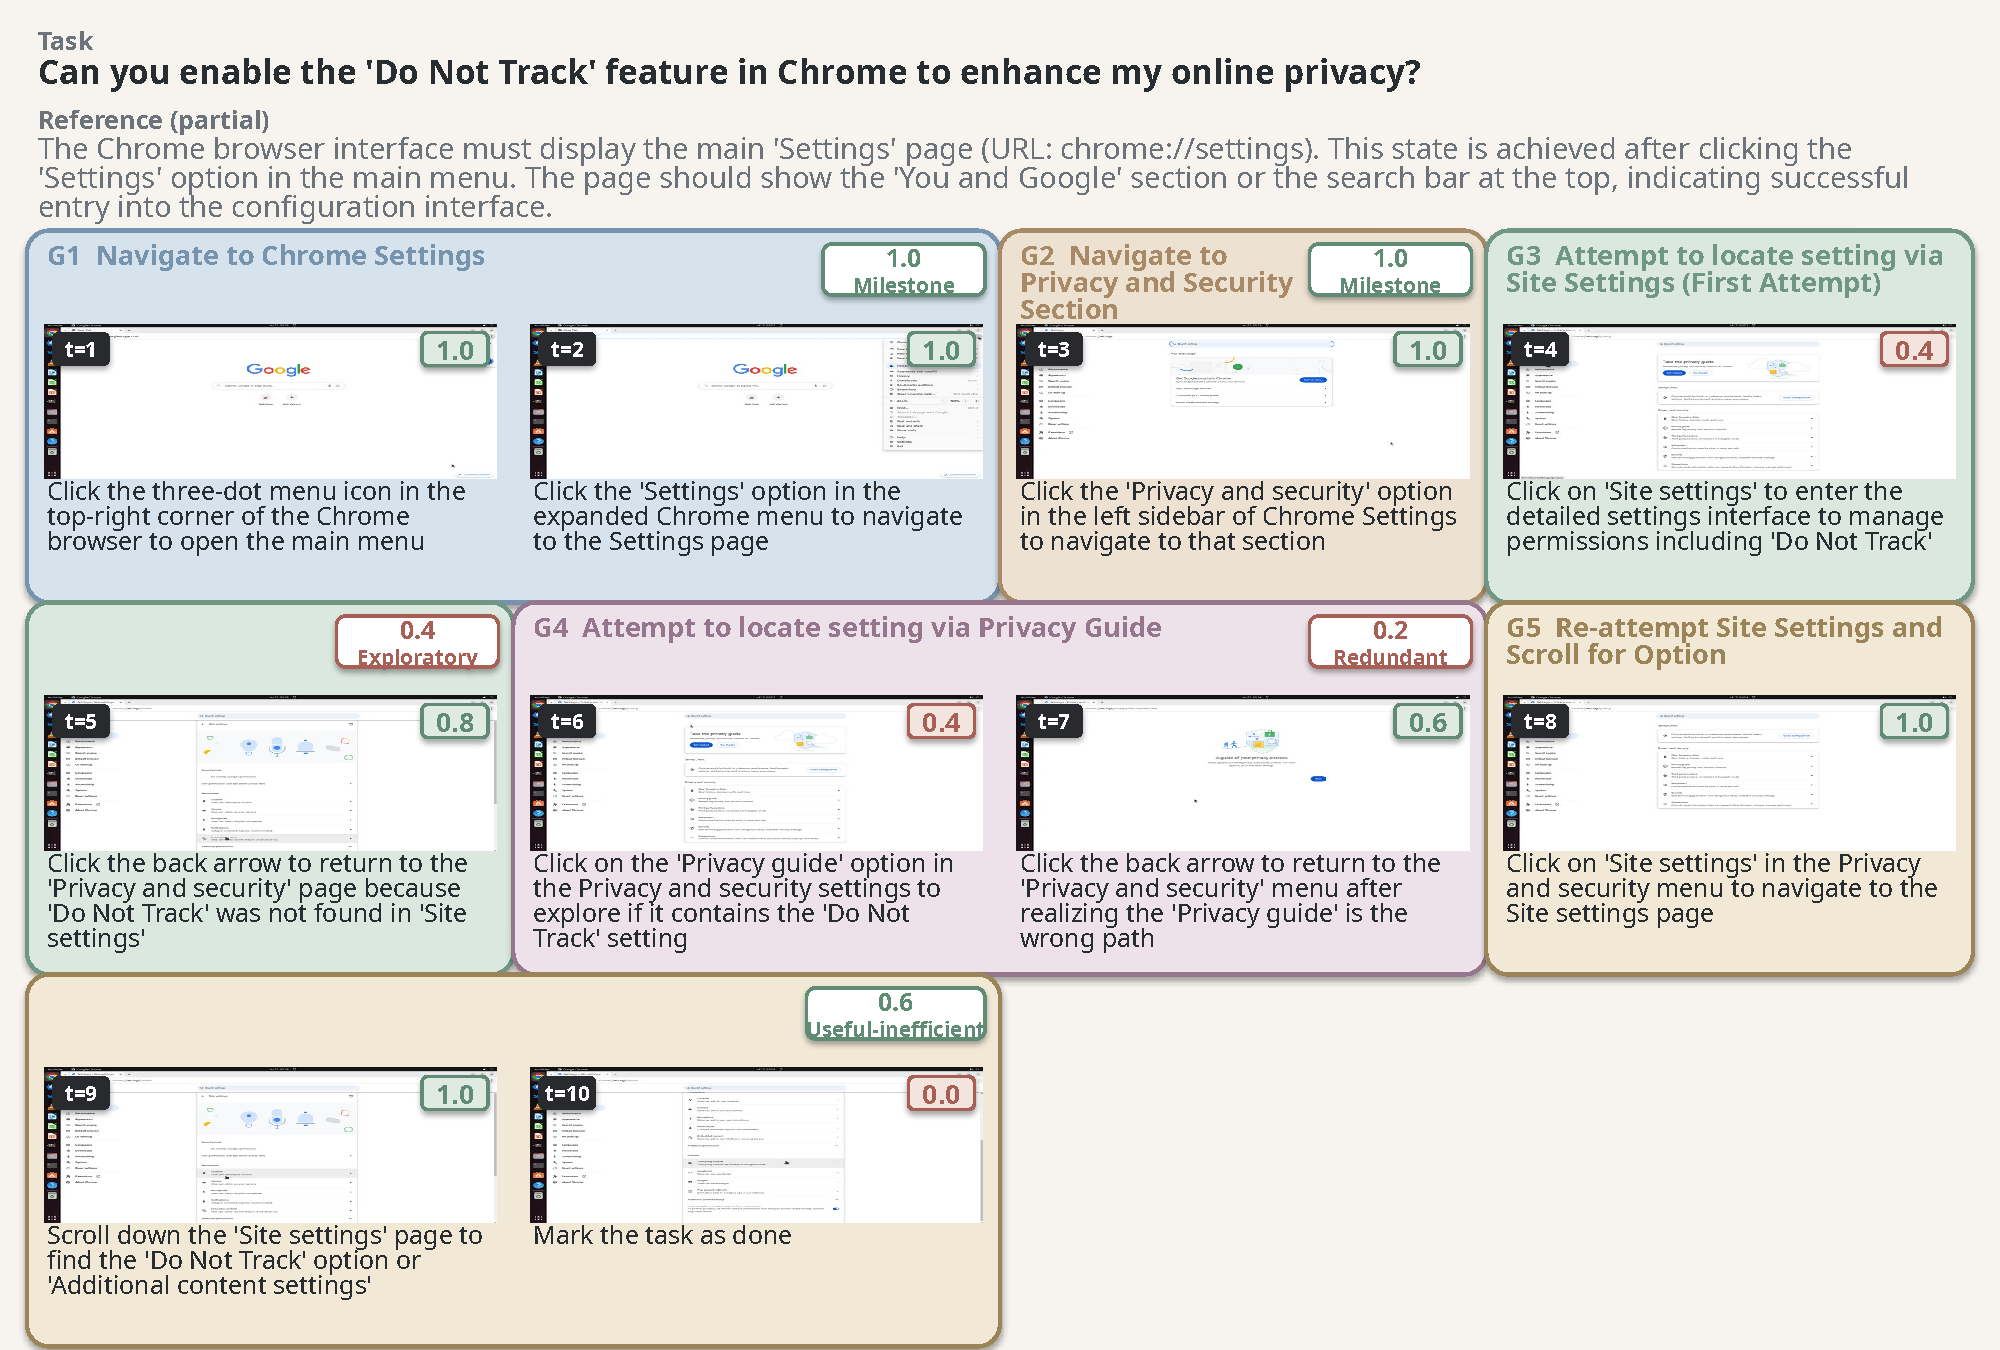
\includegraphics[width=\textwidth]{figures/qual_chrome.pdf}
\caption{A Chrome trajectory for enabling Do Not Track.}
\label{fig:qual-chrome}
\end{figure*}

Figure~\ref{fig:qual-chrome} never turns on Do Not Track, but Groups~1--2 (``Navigate to Chrome Settings'' and ``Navigate to Privacy and Security Section'') still score opening Settings and Privacy and security as useful, instead of giving every step a zero because the trajectory fails.
In Group~3, clicking ``Site settings'' is exploratory and the back arrow is Useful-efficient (it undoes the wrong page); Group~4 scores ``Privacy guide'' the same way, then lowers that group to redundant because Group~3 has already shown the setting is not there.
Group~5 scores going back to ``Site settings'' as useful, but the premature \texttt{DONE} as $0$.

\begin{figure*}[t]
\centering
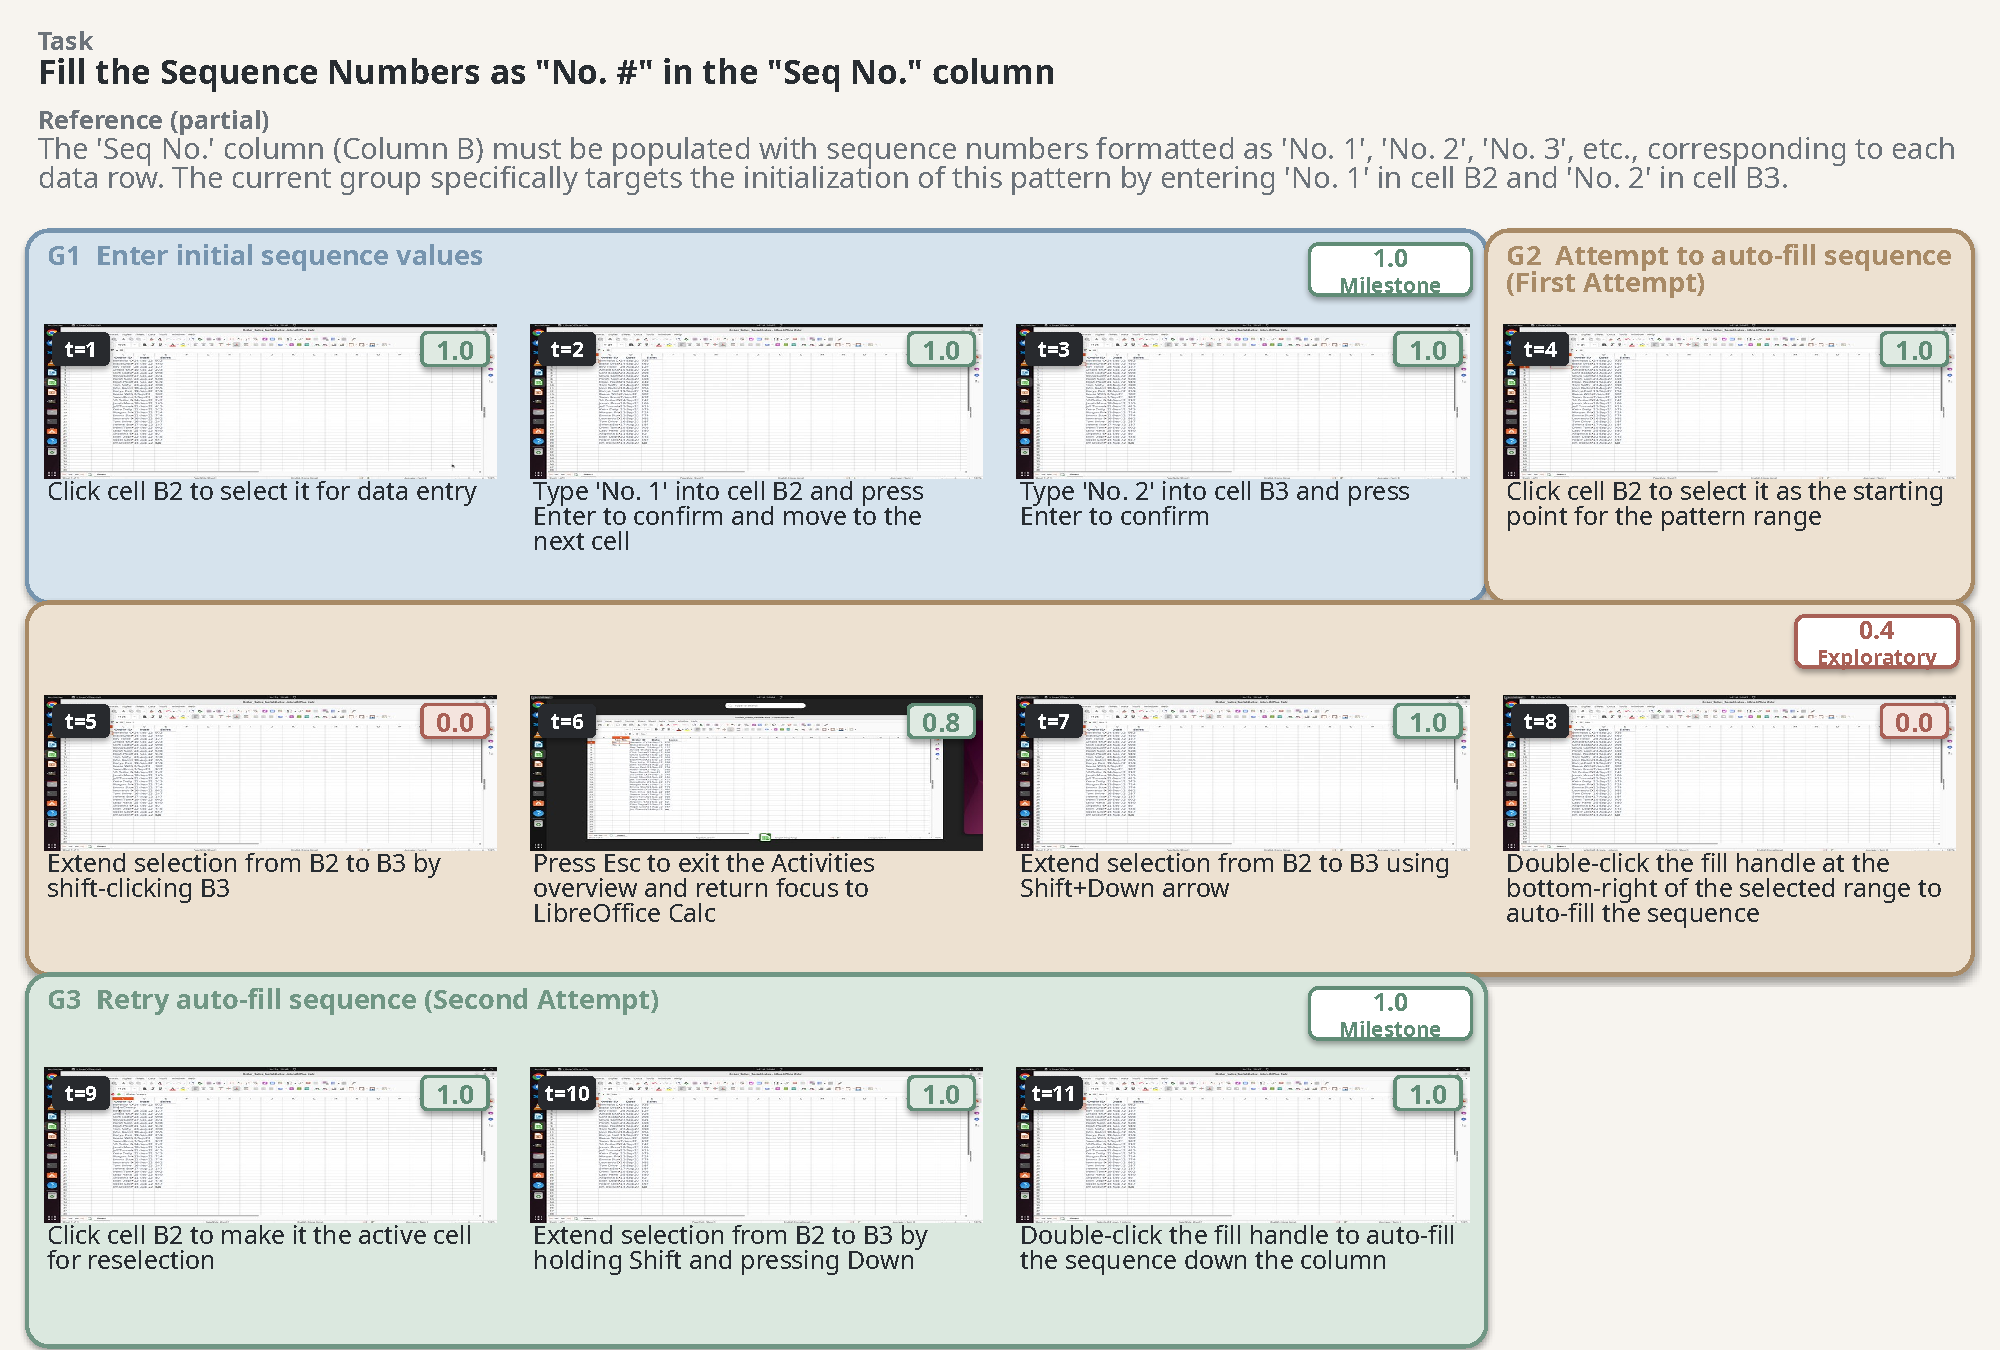
\includegraphics[width=\textwidth]{figures/qual_calc.pdf}
\caption{A Calc trajectory that fills the Seq No.\ column with ``No.\ \#''.}
\label{fig:qual-calc}
\end{figure*}

Figure~\ref{fig:qual-calc} fills the column only after Group~2 (``Attempt to auto-fill sequence (First Attempt)'') fails.
If only the final outcome were used, the misclick that opens Activities would get the same success credit as the later fill.
Grouping puts typing ``No.\ 1'' and ``No.\ 2'' in Group~1 (``Enter initial sequence values''), the failed fill in Group~2, and the retry in Group~3 (``Retry auto-fill sequence (Second Attempt)''), so the successful retry does not change the scores of the failed attempt.
In Group~2, the click that opens Activities and the missed fill handle are harmful, Esc is Useful-efficient (it closes Activities and returns to Calc), and the group stays exploratory because the column is still empty; Group~3 then scores the same fill as useful after ``No.\ \#'' appears.

\begin{figure*}[t]
\centering
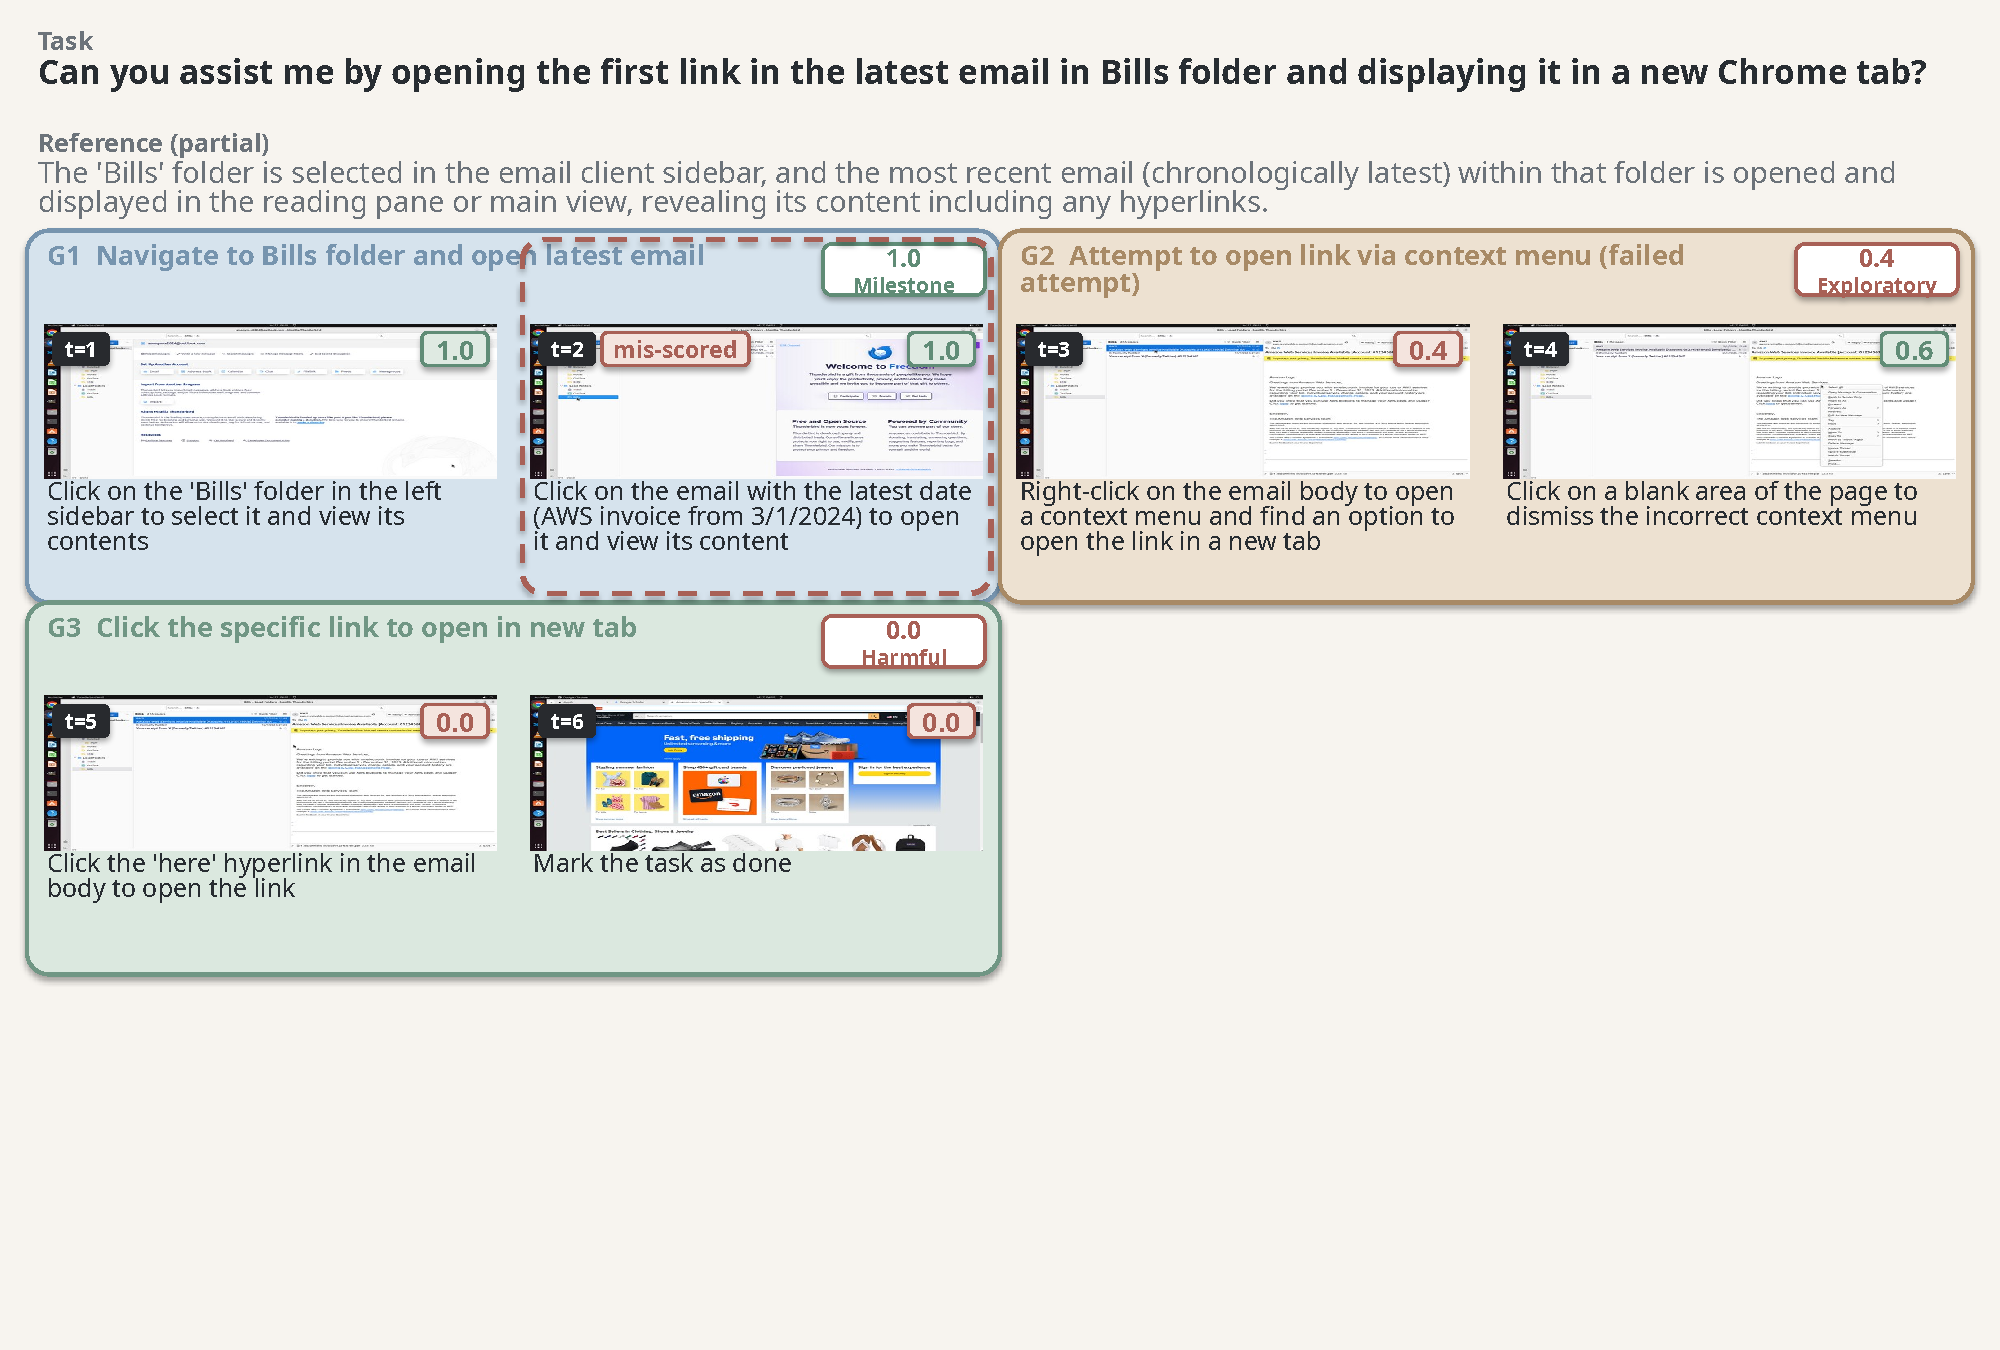
\includegraphics[width=\textwidth]{figures/qual_fail_email.pdf}
\caption{A failure-case trajectory that opens the first link in the latest Bills email in a new Chrome tab. The dashed outline marks the incorrectly scored step.}
\label{fig:qual-fail}
\end{figure*}

Figure~\ref{fig:qual-fail} shows a failure case: the process reward is wrong at the dashed step.
The instruction asks for the latest email in the Bills folder.
The list shows an AWS invoice dated $3/1/2024$ above an X receipt dated $12/1/2024$; $12/1/2024$ is later, so the second mail should be opened.
The critic compares the two dates incorrectly, treats $3/1/2024$ as newer, and scores clicking the AWS invoice as $1.0$.
This is a visual-judgment error limited by the capability of the model used as the critic: it is not reliable enough at reading a small UI detail such as which of two dates is later.
